\documentclass[tikz,border=10pt]{standalone}
\usepackage{tikz}
\usetikzlibrary{positioning,arrows.meta,shadows}

\begin{document}

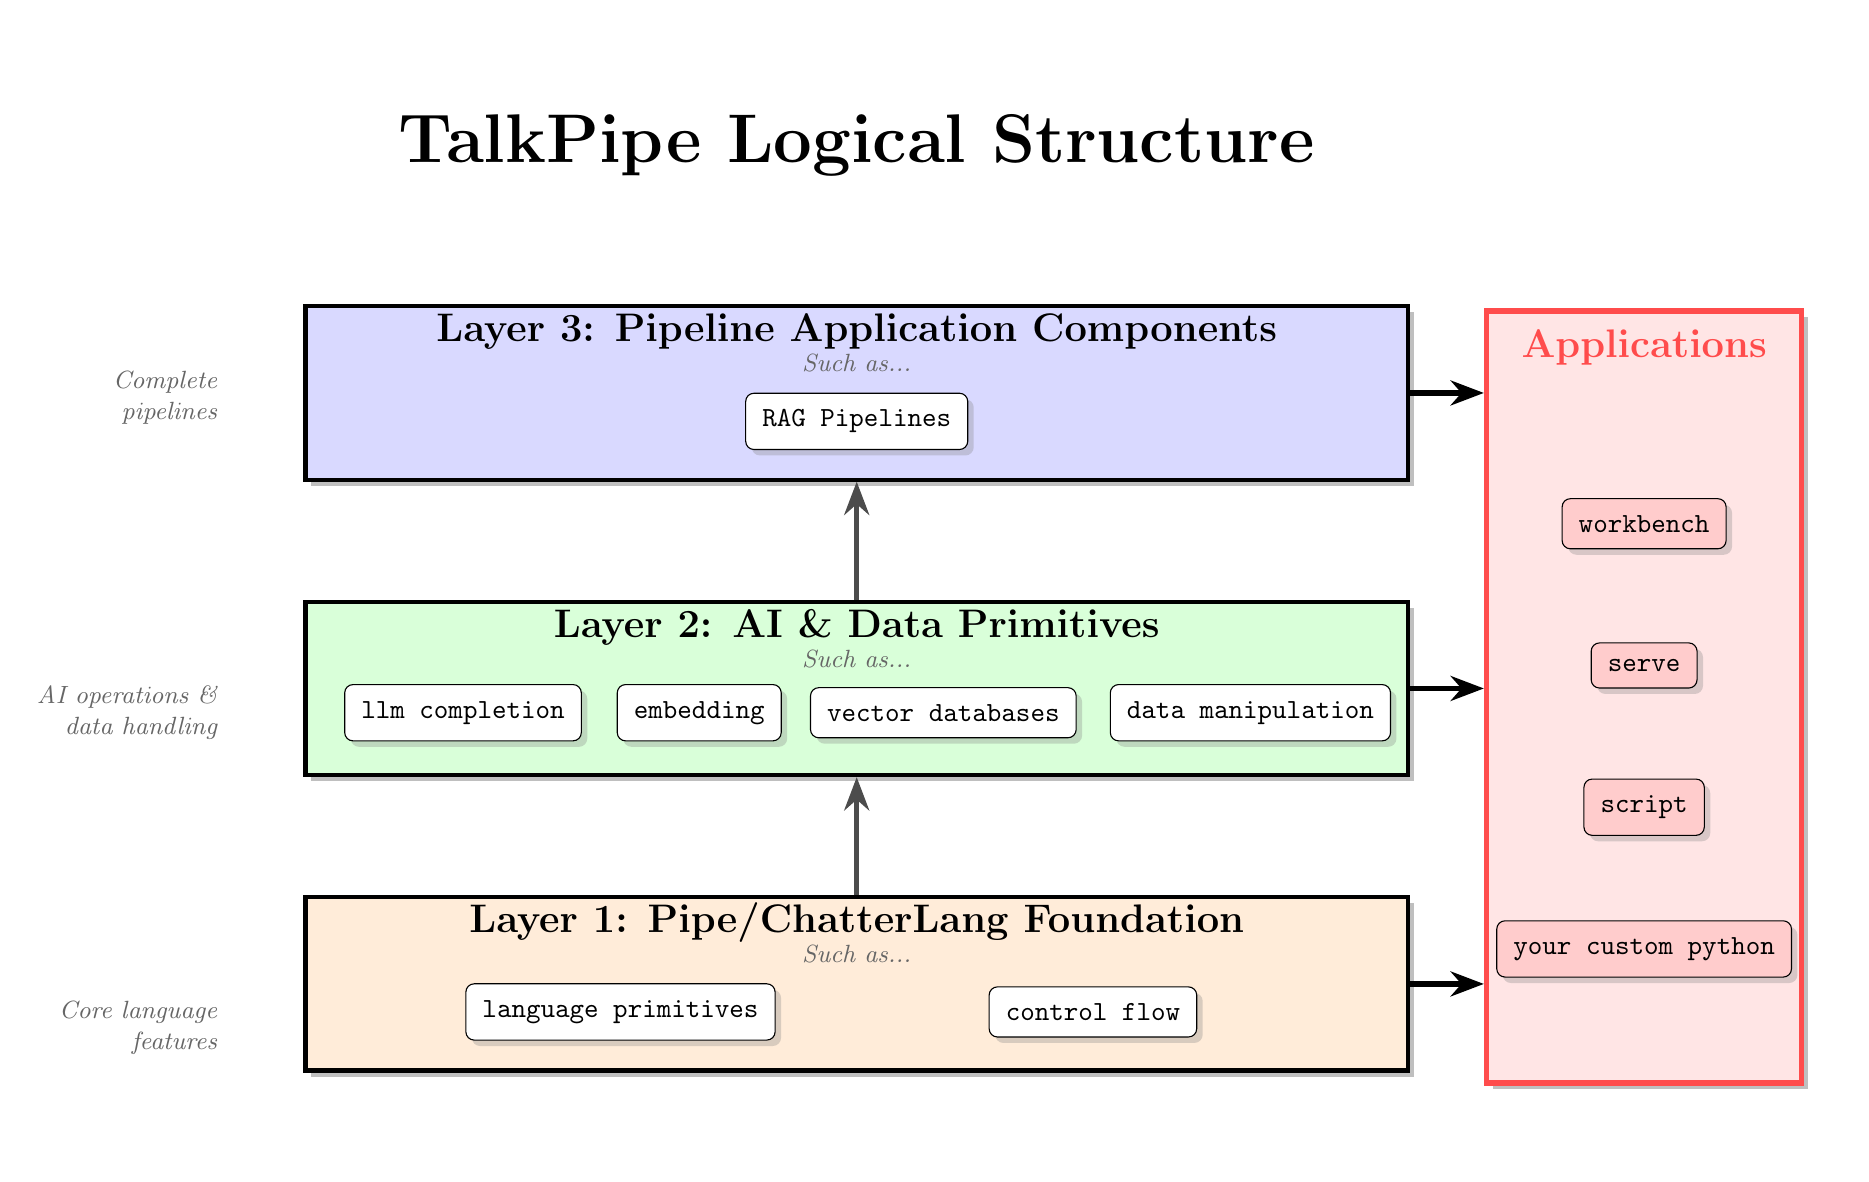
\begin{tikzpicture}[
    layer/.style={
        rectangle,
        minimum width=14cm,
        minimum height=2.2cm,
        draw=black,
        line width=1.5pt,
        drop shadow,
        font=\Large\bfseries
    },
    layertitle/.style={
        font=\Large\bfseries
    },
    component/.style={
        rectangle,
        rounded corners=3pt,
        draw=black,
        fill=white,
        inner sep=6pt,
        font=\normalsize\ttfamily,
        drop shadow={opacity=0.3}
    },
    arrow/.style={
        -Stealth,
        line width=2pt,
        draw=black!70
    }
]

% Light background for the entire diagram (for dark backgrounds)
\fill[white, rounded corners=5pt] (-10.5,1.5) rectangle (12.5,-12.8);

% Title
\node[font=\Huge\bfseries] (title) at (0,0) {TalkPipe Logical Structure};

% Layer 3 - Pipeline Components
\node[layer, fill=blue!15, below=1.5cm of title] (layer3box) {};
\node[layertitle] at (layer3box.north) [yshift=-0.35cm] {Layer 3: Pipeline Application Components};
\node[font=\small\itshape, text=black!60] at (layer3box.north) [yshift=-0.75cm] {Such as...};

\node[component] (rag) at (0,-3.5) {RAG Pipelines};

% Layer 2 - Middle Layer
\node[layer, fill=green!15, below=1.5cm of layer3box] (layer2box) {};
\node[layertitle] at (layer2box.north) [yshift=-0.35cm] {Layer 2: AI \& Data Primitives};
\node[font=\small\itshape, text=black!60] at (layer2box.north) [yshift=-0.75cm] {Such as...};

\node[component] (llm) at (-5,-7.2) {llm completion};
\node[component] (embed) at (-2.0,-7.2) {embedding};
\node[component] (vectordb) at (1.1,-7.2) {vector databases};
\node[component] (datamanip) at (5,-7.2) {data manipulation};

% Layer 1 - Bottom Layer
\node[layer, fill=orange!15, below=1.5cm of layer2box] (layer1box) {};
\node[layertitle] at (layer1box.north) [yshift=-0.35cm] {Layer 1: Pipe/ChatterLang Foundation};
\node[font=\small\itshape, text=black!60] at (layer1box.north) [yshift=-0.75cm] {Such as...};

\node[component] (prim) at (-3,-11) {language primitives};
\node[component] (control) at (3,-11) {control flow};

% Arrows showing dependency flow between layers
\draw[arrow] (layer1box.north) -- (layer2box.south);
\draw[arrow] (layer2box.north) -- (layer3box.south);

% Top-Level Applications Box on the right
% Aligned with top of layer 3 box and bottom of layer 1 box
\node[rectangle, draw=red!70, line width=2pt, fill=red!10, minimum width=4cm, minimum height=9.8cm, drop shadow] (appbox) at (10,-7.0) {};
\node[font=\Large\bfseries, text=red!70] at (appbox.north) [yshift=-0.5cm] {Applications};

\node[component, fill=red!20] (workbench) at (10,-4.8) {workbench};
\node[component, fill=red!20] (serve) at (10,-6.6) {serve};
\node[component, fill=red!20] (script) at (10,-8.4) {script};
\node[component, fill=red!20] (python) at (10,-10.2) {your custom python};

% Arrows from layers to applications box (parallel horizontal and black)
\draw[arrow, draw=black] (layer3box.east) -- (appbox.west |- layer3box.east);
\draw[arrow, draw=black] (layer2box.east) -- (appbox.west |- layer2box.east);
\draw[arrow, draw=black] (layer1box.east) -- (appbox.west |- layer1box.east);

% Side annotations
\node[anchor=east, align=right, font=\small\itshape, text=black!60] at (-8,-11.2) {Core language\\features};
\node[anchor=east, align=right, font=\small\itshape, text=black!60] at (-8,-7.2) {AI operations \&\\data handling};
\node[anchor=east, align=right, font=\small\itshape, text=black!60] at (-8,-3.2) {Complete\\pipelines};

\end{tikzpicture}

\end{document}
